% !TeX root = ../main.tex
\chapter{Background and Literature Review}
\label{ch:background}

This chapter provides the foundational knowledge and contextual background necessary to understand the HPC Sorting Serious Game. It reviews key concepts in parallel computing, serious games in education, web-based game development, and multiplayer networking architectures.

\begin{figure}[htbp]
    \centering
    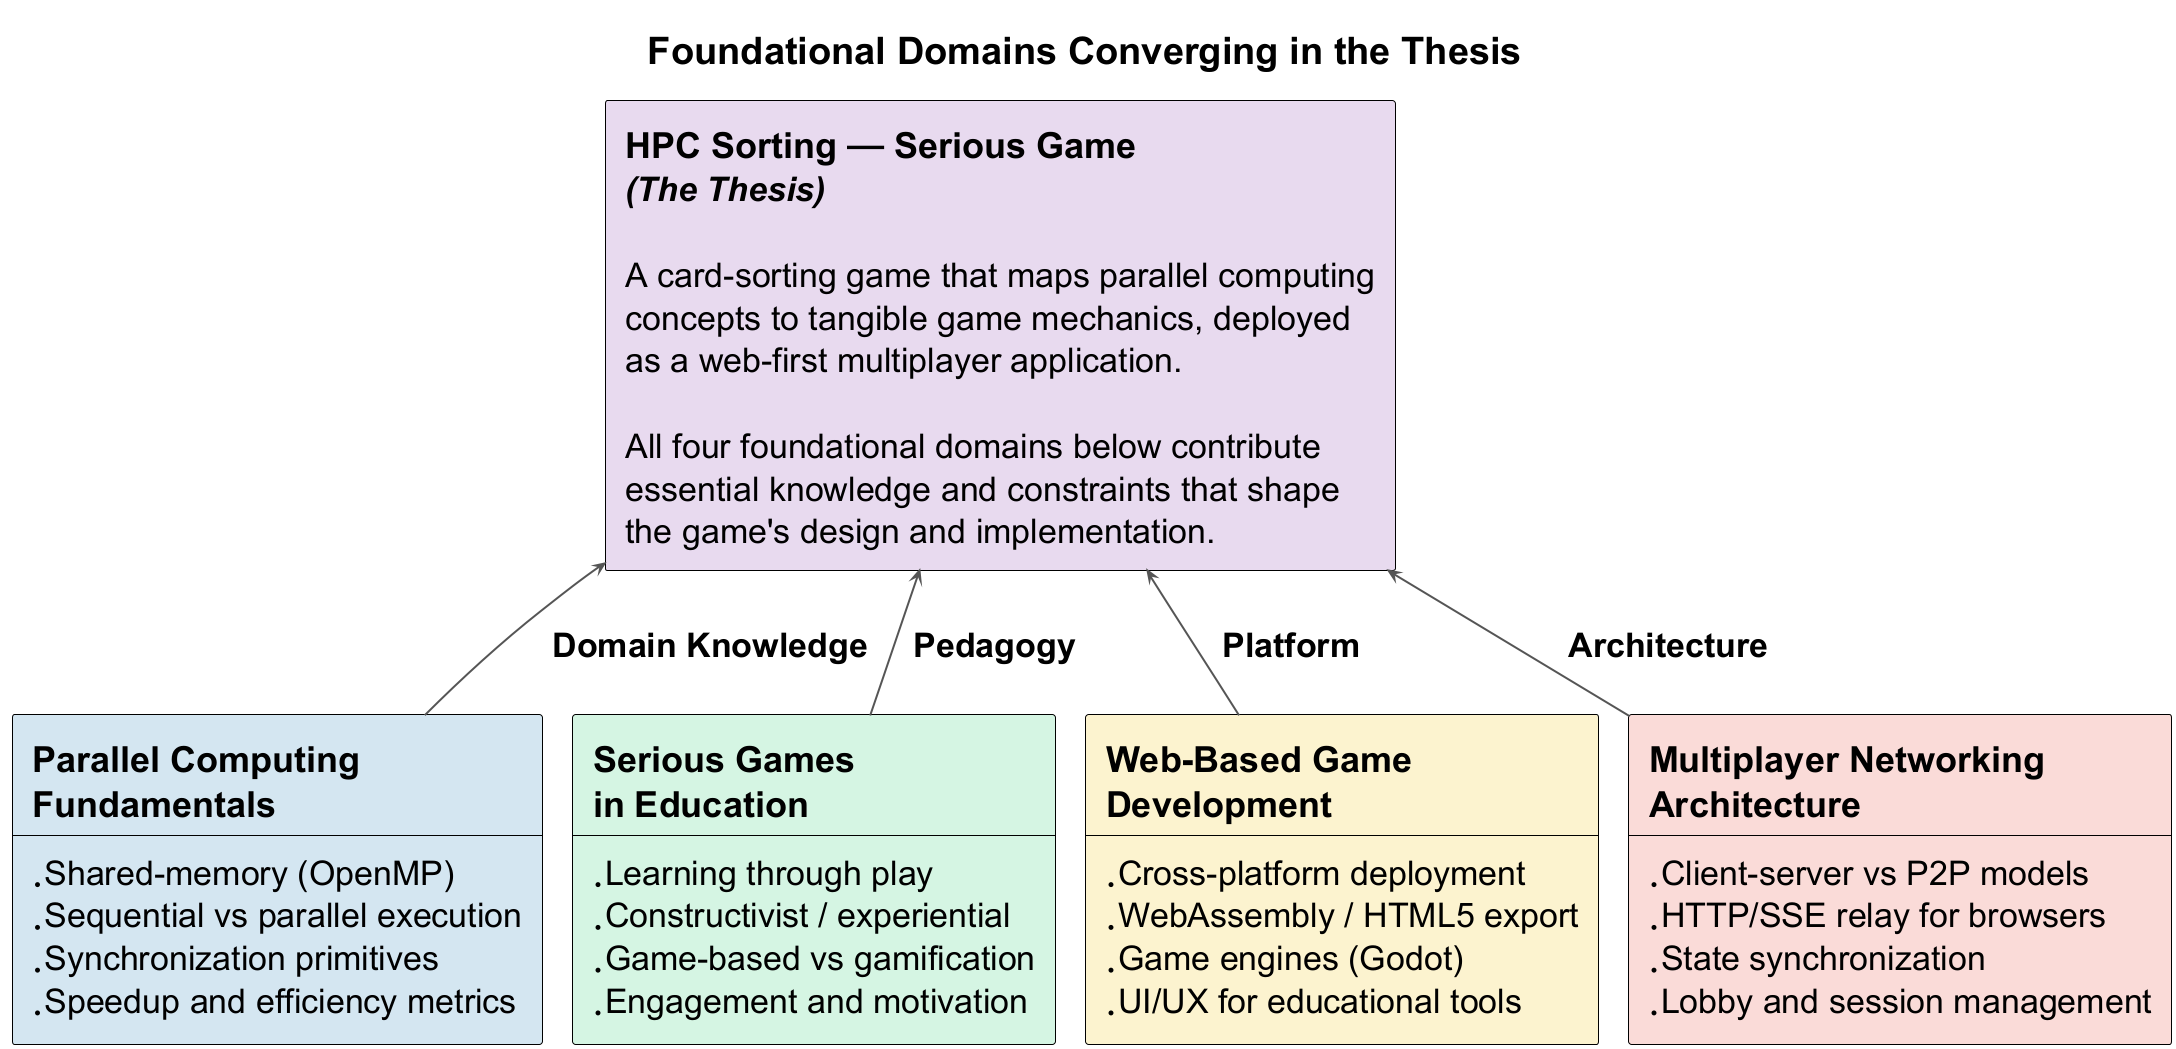
\includegraphics[width=0.95\textwidth]{figures/diagrams/background-concept-overview.png}
    \caption{Conceptual overview of the four knowledge domains converging in this thesis.}
    \label{fig:background-concept-overview}
\end{figure}

%-----------------------------------------------------------------------
\section{Parallel Computing Fundamentals}
\label{sec:parallel-computing}

Parallel computing is the simultaneous execution of multiple computational tasks to solve problems more efficiently than sequential processing. As Moore's Law approaches its physical limits, parallel computing has become essential for improving computational performance across scientific computing, data analytics, and real-time systems.

%-----------------------------------------------------------------------
\subsection{Parallel Programming Paradigms}
\label{subsec:parallel-paradigms}

Two primary paradigms dominate parallel computing education and practice: shared-memory parallelism and distributed-memory parallelism.

\subsubsection*{Shared-Memory Parallelism}

In shared-memory systems, multiple processors or cores access a common address space. All threads can read and write to the same memory locations, enabling efficient data sharing but requiring careful synchronization to prevent race conditions.

\textbf{Characteristics:}
\begin{itemize}
    \item All processors access the same physical memory
    \item Communication between threads occurs through shared variables
    \item Synchronization primitives (locks, barriers, atomic operations) prevent conflicts
    \item Lower communication overhead compared to distributed memory
    \item Scalability typically limited to a single workstation (one multi-core node)
\end{itemize}

\textbf{Applications:} Shared-memory parallelism is ideal for problems requiring frequent communication between processing units, such as iterative algorithms, graph processing, and data analytics on multicore processors.

\subsubsection*{Distributed-Memory Parallelism}

In distributed-memory systems, each processor has its own local memory. Processors communicate by explicitly sending and receiving messages over a network, requiring programmers to manage data distribution and communication patterns.

\textbf{Characteristics:}
\begin{itemize}
    \item Each processor has private memory space
    \item Communication between processes requires explicit message passing
    \item Scalable to thousands or millions of processors
    \item Higher communication overhead and latency
    \item No shared state eliminates race conditions but complicates programming
\end{itemize}

\textbf{Applications:} Distributed-memory parallelism is essential for large-scale scientific simulations, weather modeling, molecular dynamics, and big data processing across cluster and supercomputer architectures.

%-----------------------------------------------------------------------
\subsection{OpenMP: Shared-Memory Programming}
\label{subsec:openmp}

OpenMP (Open Multi-Processing) is a widely-used API for shared-memory parallel programming in C, C++, and Fortran. It uses compiler directives (pragmas) to specify parallel regions, enabling incremental parallelization of sequential code.

\textbf{Core Concepts:}
\begin{enumerate}
    \item \textbf{Parallel Regions}: Code sections executed by multiple threads simultaneously
    \item \textbf{Work-Sharing Constructs}: Distribute loop iterations or tasks among threads
    \item \textbf{Data Scoping}: Variables can be shared (visible to all threads) or private (thread-local copies)
    \item \textbf{Synchronization}: Barriers, critical sections, and atomic operations coordinate thread execution
    \item \textbf{Scheduling}: Strategies (static, dynamic, guided) control how iterations are assigned to threads
\end{enumerate}

\paragraph*{Example Code:}

\begin{lstlisting}[language=C++, caption={Simple OpenMP parallel loop}]
#pragma omp parallel for schedule(dynamic)
for (int i = 0; i < N; i++) {
    array[i] = compute_value(i);
}
\end{lstlisting}

\textbf{Educational Value:} OpenMP's simplicity makes it excellent for teaching parallel programming concepts. The incremental approach—starting with sequential code and adding pragmas—allows students to observe immediate performance improvements while learning about thread management, data dependencies, and race conditions.

%-----------------------------------------------------------------------
\subsection{MPI: Distributed-Memory Programming}
\label{subsec:mpi}

\begin{mdframed}[backgroundcolor=yellow!10, linecolor=orange, linewidth=2pt]
    \textbf{Note:} This section provides background on MPI for completeness and context within the broader HPC landscape. \textbf{The game implemented in this thesis focuses exclusively on OpenMP shared-memory parallelism.} MPI distributed-memory concepts are discussed here for educational context but are \textbf{not implemented} in the current version. See Chapter~\ref{ch:conclusion} for discussion of MPI as potential future work.
\end{mdframed}

MPI (Message Passing Interface) is the de facto standard for distributed-memory parallel programming. It provides a rich set of communication primitives for sending and receiving messages between processes, enabling scalable parallel computing on clusters and supercomputers.

\textbf{Core Operations:}
\begin{description}
    \item[Point-to-Point Communication] \texttt{MPI\_Send} and \texttt{MPI\_Recv} exchange messages between specific processes
    \item[Collective Communication] Operations like \texttt{MPI\_Bcast}, \texttt{MPI\_Gather}, and \texttt{MPI\_Reduce} involve all processes in a communicator
    \item[Process Groups] Communicators organize processes and define communication contexts
    \item[Data Types] MPI supports both primitive and user-defined data types for message content
\end{description}

\paragraph*{Example Code:}

\begin{lstlisting}[language=C++, caption={Simple MPI message passing}]
MPI_Init(&argc, &argv);
int rank, size;
MPI_Comm_rank(MPI_COMM_WORLD, &rank);
MPI_Comm_size(MPI_COMM_WORLD, &size);

if (rank == 0) {
    // Master process
    MPI_Send(data, count, MPI_INT, 1, 0, MPI_COMM_WORLD);
} else if (rank == 1) {
    // Worker process
    MPI_Recv(data, count, MPI_INT, 0, 0, MPI_COMM_WORLD, &status);
}

MPI_Finalize();
\end{lstlisting}

\textbf{Educational Value:} MPI teaches students about distributed computing challenges including data distribution, explicit communication, latency management, and scalability. The message-passing model forces programmers to think carefully about data ownership and communication patterns, skills essential for modern distributed systems.

%-----------------------------------------------------------------------
\subsection{Parallel Sorting Algorithms}
\label{subsec:parallel-sorting}

Sorting is a fundamental algorithmic problem that benefits significantly from parallelization. Several parallel sorting strategies exist, each with different communication and synchronization requirements.

\paragraph*{Parallel Merge Sort:}
\begin{itemize}
    \item Recursively divide array into subarrays
    \item Sort subarrays in parallel
    \item Merge sorted subarrays (potentially in parallel)
    \item Well-suited for shared-memory systems
    \item Time complexity: $O(\frac{n \log n}{p})$ with $p$ processors
\end{itemize}

\paragraph*{Parallel Quicksort:}
Parallel quicksort \citep{sanders2019sequential} exploits task-level parallelism through its recursive divide-and-conquer structure:
\begin{itemize}
    \item Select a \emph{pivot} element from the array
    \item \textbf{Partition} the array: elements $\leq$ pivot go left, elements $>$ pivot go right
    \item Recursively sort the left and right partitions \emph{in parallel} (each assigned to a different thread/task)
    \item Quality of the pivot determines load balance---a poor pivot creates unequal partitions
    \item Expected time complexity: $O\!\left(\frac{n \log n}{p}\right)$ with $p$ processors, assuming balanced pivots
\end{itemize}
Unlike merge sort, where the \emph{merge} phase is the synchronization bottleneck, quicksort's challenge is the \emph{partition} phase: threads must agree on a pivot and redistribute data before independent recursion can proceed. Parallel partitioning schemes (e.g., each thread partitions a local block, then a prefix-sum determines final positions) can parallelize this step, but at the cost of additional communication \citep{sanders2019sequential}.

\paragraph*{Sample Sort (MPI Pattern):}
\begin{itemize}
    \item Distribute data across processes
    \item Each process sorts local data
    \item Select sample elements to determine global pivots
    \item Redistribute data based on pivots
    \item Each process sorts its final partition
    \item Commonly used in distributed-memory systems
    \item \textit{Note: Not implemented in this thesis; discussed for context}
\end{itemize}

\textbf{Relevance to Educational Game:} The card-sorting game mechanics map directly to parallel sorting algorithms \citep{sanders2019sequential}. \emph{Parallel merge sort} maps to the game's divide-into-buffers, sort-locally, then merge-back workflow, with barriers separating each merge round. \emph{Parallel quicksort} maps to collaborative pivot selection and partitioning, followed by sub-group recursion into smaller card sub-arrays. In the implemented game, players act as threads (OpenMP) coordinating through shared memory to sort cards efficiently, making abstract algorithmic concepts tangible through gameplay. Chapter~\ref{ch:architecture} demonstrates how the existing algorithm-agnostic architecture already supports both strategies without code changes, and Chapter~\ref{ch:conclusion} outlines potential guided modes as medium-term extensions.

%-----------------------------------------------------------------------
\section{Serious Games in Education}
\label{sec:serious-games}

Serious games—games designed primarily for purposes beyond entertainment—have emerged as powerful educational tools. This section reviews the theoretical foundations and empirical evidence supporting game-based learning.

%-----------------------------------------------------------------------
\subsection{Definition and Characteristics}
\label{subsec:serious-games-definition}

\citet{zyda2005visual} defines a serious game as ``a mental contest, played with a computer in accordance with specific rules, that uses entertainment to further \textelp{} training, education, health, public policy, and strategic communication objectives.'' These games leverage game design principles to achieve learning objectives, skill development, or behavioral change.

\textbf{Key Characteristics:}
\begin{itemize}
    \item \textbf{Clear Learning Objectives}: Explicit educational goals aligned with curricula
    \item \textbf{Engaging Mechanics}: Game elements (challenges, rewards, feedback) maintain motivation
    \item \textbf{Active Learning}: Players learn by doing, not passive observation
    \item \textbf{Immediate Feedback}: Instant consequences of actions reinforce learning
    \item \textbf{Safe Experimentation}: Risk-free environment for trial and error
    \item \textbf{Progressive Difficulty}: Challenges scale with player skill development
\end{itemize}

%-----------------------------------------------------------------------
\subsection{Theoretical Foundations}
\label{subsec:game-based-learning-theory}

Game-based learning draws on several established educational theories:

\paragraph*{Constructivism:}

Constructivist theory \citep{piaget1970genetic} posits that learners actively construct knowledge through experience rather than passively receiving information. Games naturally support constructivist learning by placing players in problem-solving scenarios where they discover principles through experimentation.

\paragraph*{Flow Theory:}

\citet{csikszentmihalyi1990flow} describes ``flow'' as the optimal psychological state where challenge level matches skill level, producing deep engagement. Well-designed educational games maintain flow by dynamically adjusting difficulty, keeping learners challenged without overwhelming them.

\paragraph*{Experiential Learning:}

\citet{kolb1984experiential}'s experiential learning cycle---concrete experience, reflective observation, abstract conceptualization, active experimentation---aligns naturally with game mechanics. Players experience situations, observe outcomes, form hypotheses, and test them iteratively.

%-----------------------------------------------------------------------
\subsection{Empirical Evidence}
\label{subsec:serious-games-evidence}

Research consistently demonstrates the effectiveness of serious games for learning:

\paragraph*{\citet{connolly2012systematic} Meta-Analysis:}

A systematic literature review analysing 70 empirical studies found that serious games positively impact learning outcomes across multiple domains. Key findings include:

\begin{itemize}
    \item Improved knowledge acquisition and retention
    \item Enhanced perceptual and cognitive skills
    \item Increased motivation and engagement
    \item Better affective and motivational outcomes
    \item Most effective when integrated with traditional instruction
\end{itemize}

\paragraph*{\citet{papastergiou2009digital} Computer Science Education:}

A study of digital game-based learning in high school computer science found that students using educational games demonstrated:

\begin{itemize}
    \item Significantly higher knowledge acquisition
    \item Greater enjoyment and motivation
    \item Preference for game-based learning over traditional methods
    \item Improved attitudes toward computer science
\end{itemize}

%-----------------------------------------------------------------------
\subsection{Serious Games in Computer Science}
\label{subsec:games-cs-education}

Several successful serious games target computer science education.
\textbf{CodeCombat} \citep{codecombat} teaches programming through RPG-style gameplay in which players write real Python or JavaScript code to control characters; it is used in thousands of classrooms worldwide.
\textbf{Lightbot} \citep{lightbot} introduces sequencing, loops, and procedures through a visual puzzle interface that requires no programming syntax, making it accessible to young learners.

\paragraph*{Parallel Computing Games:}

In contrast to introductory programming, very few serious games target advanced topics like parallel computing education. Instructors typically rely on traditional, non-gamified software visualizers or simulation tools to teach parallel algorithm design, highlighting a significant gap in the current game-based learning landscape for advanced computer science topics.

%-----------------------------------------------------------------------
\subsection{Serious Games for HPC Education}
\label{subsec:serious-games-hpc}

High Performance Computing education faces unique challenges that serious games can address:

\paragraph*{Why Games for HPC?}

\begin{enumerate}
    \item \textbf{Abstract Concepts}: HPC involves invisible processes (threads, messages, synchronization) that are difficult to visualize through static diagrams
    \item \textbf{Temporal Dynamics}: Parallelism involves timing, race conditions, and coordination that unfold over time---games naturally model dynamic systems
    \item \textbf{Scale Mismatch}: Real HPC systems involve millions of operations per second; games can slow down and make these concepts observable
    \item \textbf{Hands-On Experience}: Students learn parallelism best by experiencing coordination challenges firsthand
\end{enumerate}

\paragraph*{Mapping HPC Concepts to Game Mechanics:}
The following mappings enable intuitive understanding of HPC concepts through gameplay (see Table~\ref{tab:hpc-game-mapping}).

\begin{table}[htbp]
    \centering
    \caption{HPC concepts mapped to game mechanics}
    \label{tab:hpc-game-mapping}
    \begin{tabular}{@{}l|l@{}}
        \toprule
        \textbf{HPC Concept}   & \textbf{Game Mechanic}                   \\
        \midrule
        Threads/Processes      & Players                                  \\
        \midrule
        Shared Memory          & Shared game board/container              \\
        \midrule
        Thread-Local Storage   & Private player inventory                 \\
        \midrule
        Synchronization        & Turn-taking or barriers                  \\
        \midrule
        Race Conditions        & Conflicting simultaneous actions         \\
        \midrule
        Speedup                & Time comparison (1 player vs. N players) \\
        \midrule
        Communication Overhead & Time to transfer items between players   \\
        \midrule
        Load Balancing         & Equal distribution of work               \\
        \bottomrule
    \end{tabular}
\end{table}

\paragraph*{Advantages of Game-Based HPC Learning:}

\begin{itemize}
    \item \textbf{No Prerequisites}: Students can experience parallel concepts before learning programming syntax
    \item \textbf{Misconception Surfacing}: Games reveal incorrect mental models (e.g., ``more threads always faster'')
    \item \textbf{Quantifiable Learning}: Performance metrics (time, moves) provide concrete feedback
    \item \textbf{Collaborative Learning}: Multiplayer games naturally create discussion and peer learning
    \item \textbf{Scalable Delivery}: Web-based games reach students regardless of institutional HPC infrastructure
\end{itemize}

%-----------------------------------------------------------------------
\section{Web-Based Game Development}
\label{sec:web-game-dev}

Web browsers provide a universal platform for educational game deployment, eliminating installation barriers and enabling access from any device with a modern browser.

%-----------------------------------------------------------------------
\subsection{Web Platform Advantages}
\label{subsec:web-advantages}

\textbf{Accessibility:} Web games require no installation—students access the game via URL, eliminating software distribution challenges and platform compatibility concerns.

\textbf{Cross-Platform:} A single web build runs on Windows, macOS, Linux, and even mobile browsers, maximizing reach with minimal development overhead.

\textbf{Instant Updates:} Deploying updates is immediate—no app store approval processes or user-initiated updates required.

\textbf{Low Barrier:} Modern browsers include powerful JavaScript engines, WebGL for graphics, and APIs for real-time communication.

%-----------------------------------------------------------------------
\subsection{Web Development Challenges}
\label{subsec:web-challenges}

\textbf{Browser Sandboxing:} Security restrictions prevent raw socket access, UDP communication, and local peer discovery—complicating multiplayer networking.

\textbf{Performance Overhead:} WebAssembly and JavaScript have overhead compared to native code, though performance is acceptable for 2D games.

\textbf{Networking Limitations:} Traditional peer-to-peer networking (like WebRTC data channels) can be complex to configure and may not work reliably across all network configurations.

%-----------------------------------------------------------------------
\subsection{Game Engines for Web}
\label{subsec:web-game-engines}

Several game engines support web deployment through HTML5/WebAssembly export, each with different trade-offs relevant to educational game development:
%TODO add links!
\begin{description}
    \item[Unity] offers a mature ecosystem with extensive documentation and asset store, but web exports tend to be large (50--100~MB) and the licensing model introduces constraints for open-source educational projects.
    \item[Unreal Engine] provides advanced rendering and networking capabilities; however, its focus on high-fidelity 3D and large export sizes make it less suited for lightweight 2D browser applications.
    \item[Godot Engine] is fully open-source (MIT license), produces compact web exports, and provides a Python-like scripting language (GDScript) alongside a scene-based architecture oriented toward rapid 2D development.
    \item[Cocos2d] is efficient for 2D applications and supports cross-platform builds, though its tooling ecosystem is smaller and the editor workflow is less integrated than some alternatives.
\end{description}

Key evaluation criteria for an educational web game include export size (affecting load time), 2D rendering quality, scripting accessibility for students who may inspect source code, and licensing compatibility with open educational resources. The engine selection process, evaluation evidence, and final decision are presented in Chapter~\ref{ch:methodology}, Section~\ref{subsec:godot-selection}.

%-----------------------------------------------------------------------
\section{Multiplayer Game Architecture}
\label{sec:bg-multiplayer-architecture}

Multiplayer functionality is essential for simulating OpenMP shared-memory parallelism with multiple players collaborating on shared data. This section reviews common multiplayer architectures and networking technologies.

\begin{figure}[htbp]
    \centering
    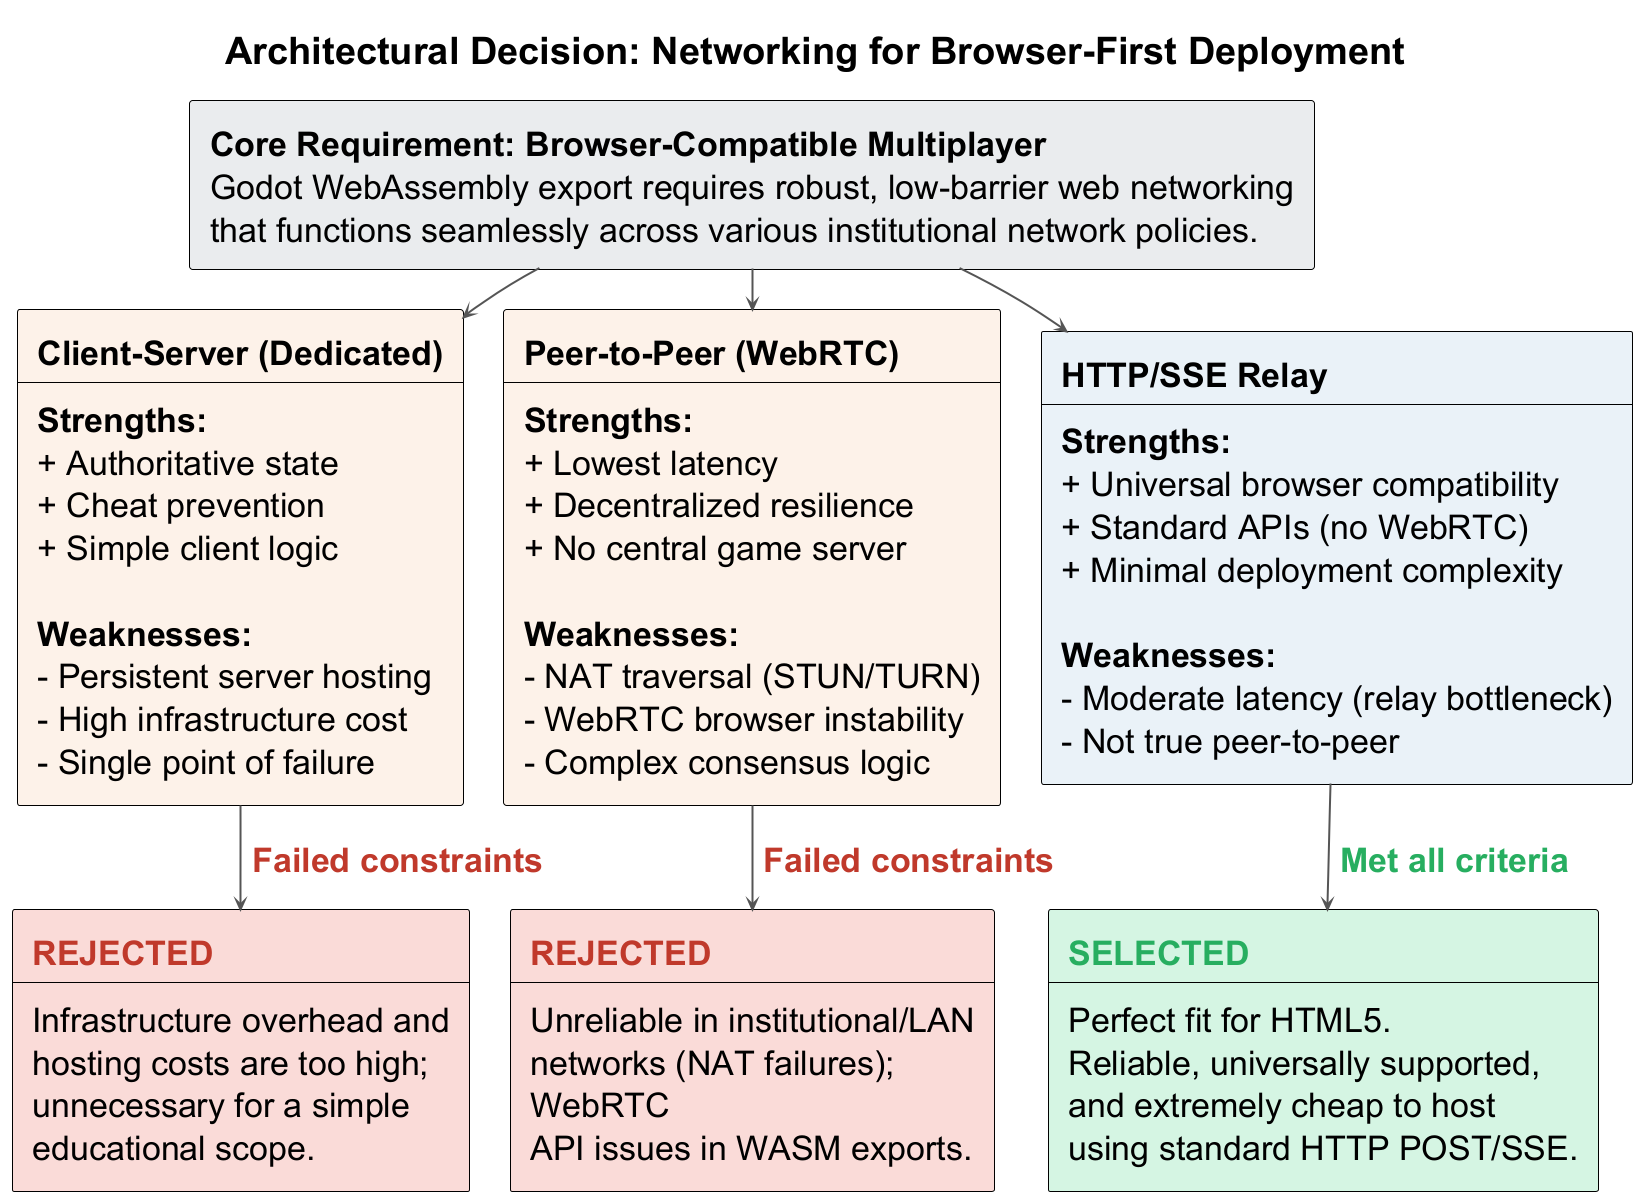
\includegraphics[width=0.95\textwidth]{figures/diagrams/networking-approach-comparison}
    \caption{Comparison of networking approaches for browser-first deployment, highlighting the HTTP/SSE relay selected for this thesis.}
    \label{fig:networking-approach-comparison}
\end{figure}

\begin{table}[htbp]
    \centering
    \caption{Summary matrix of networking approach evaluation criteria}
    \label{tab:networking-approach-summary}
    \small
    \begin{tabular}{@{}p{0.28\textwidth}p{0.2\textwidth}p{0.2\textwidth}p{0.2\textwidth}@{}}
        \toprule
        \textbf{Evaluation Criteria} & \textbf{Client-Server} & \textbf{P2P (WebRTC)} & \textbf{HTTP/SSE Relay} \\
        \midrule
        Browser compatibility        & Partial                & Problematic           & \textbf{Universal}      \\
        Infrastructure needs         & High                   & Low (STUN/TURN)       & \textbf{Minimal}        \\
        Implementation complexity    & Medium                 & High                  & \textbf{Low}            \\
        Latency                      & Low                    & Lowest                & Moderate                \\
        \bottomrule
    \end{tabular}
\end{table}

%-----------------------------------------------------------------------
\subsection{Client-Server Architecture}
\label{subsec:client-server}

In a traditional client-server model, a dedicated server hosts the authoritative game state. Clients send their inputs to the server, which validates actions, updates the canonical state, and broadcasts the result to all connected clients. This architecture provides strong consistency guarantees and inherent cheat prevention, since no client can unilaterally alter the game state. However, it requires maintaining dedicated server infrastructure, introduces a single point of failure, and routes all communication through the server, adding latency to every interaction. These costs are justified in scenarios where state correctness is paramount, but they impose operational overhead that may be disproportionate for small-scale educational deployments.

%-----------------------------------------------------------------------
\subsection{Peer-to-Peer Architecture}
\label{subsec:p2p}

Peer-to-peer (P2P) networks eliminate the need for a dedicated server by allowing clients to communicate directly. One peer is typically designated as ``host'' to serve as the authority for conflict resolution. This approach removes server infrastructure costs and can reduce latency for direct connections between nearby peers. However, establishing connections is considerably more complex due to NAT traversal requirements, and the host peer bears a disproportionate performance burden. Cheat prevention is also more difficult, since clients have more control over state. P2P topologies scale well for small groups (2--8 players) but become impractical as group size increases due to the quadratic growth in connection count.

%-----------------------------------------------------------------------
\subsection{Web Transport Technologies}
\label{subsec:web-transport}

Web browsers offer several options for real-time communication, each with trade-offs:

\paragraph*{HTTP Polling} is the simplest approach: the client repeatedly requests updates from the server at fixed intervals. It is universally supported and trivial to implement, but incurs higher latency and server load due to the frequency of requests, making it suitable only for low-frequency state updates.

\paragraph*{Server-Sent Events (SSE)} allow the server to push events to the client over a persistent HTTP connection. SSE is simpler than WebSocket (it uses standard HTTP with no protocol upgrade), supports automatic reconnection through the browser API, and enjoys broad proxy compatibility. The trade-off is that the channel is unidirectional---server to client only---so client-to-server communication must use a separate mechanism such as HTTP POST.

\paragraph*{HTTP + SSE Relay Architecture:}

For web-based multiplayer games requiring broad browser compatibility, a relay server architecture using HTTP POST for client-to-server communication and SSE for server-to-client events provides:

\begin{itemize}
    \item Universal browser support without WebSocket complexity
    \item Works through firewalls and proxies that block WebSocket
    \item Simplified connection establishment (no STUN/TURN required)
    \item Trade-off: All traffic routes through server (no P2P)
    \item Acceptable latency for turn-based or slower-paced games
\end{itemize}

%-----------------------------------------------------------------------
\subsection{State Synchronization Patterns}
\label{subsec:state-sync}

Maintaining consistent game state across multiple clients is challenging. Common patterns include:

\paragraph*{Deterministic Lockstep}
requires all clients to simulate identical game logic, with inputs synchronized and executed simultaneously. This guarantees identical state on every client but is highly sensitive to latency and packet loss, making it most suitable for real-time strategy games (e.g., \textit{Age of Empires}, \textit{StarCraft}).

\paragraph*{Client-Side Prediction}
allows clients to predict the results of their own actions immediately, while the server validates and corrects if necessary. This provides a responsive feel despite latency, at the cost of occasional reconciliation when predictions are wrong. First-person shooters such as \textit{Counter-Strike} and \textit{Overwatch} rely on this technique.

\paragraph*{Authoritative Server/Host}
models maintain a single canonical state on the server or host. Clients send proposed actions and receive authoritative state updates in return. This approach is simpler to implement and reason about, provides stronger consistency, and is well-suited for turn-based or slower-paced games where moderate latency is acceptable.

\paragraph*{Suitability for Educational Games:}

For educational multiplayer games where correctness and pedagogical clarity take priority over competitive low-latency performance, the \textbf{authoritative server/host} model is a natural fit: it is straightforward to implement, prevents inconsistencies across clients, and aligns with centralized coordination patterns found in parallel computing. The specific synchronization model adopted for this thesis is discussed in Chapter~\ref{ch:methodology}.

%-----------------------------------------------------------------------
\section{Related Work}
\label{sec:related-work}

This section reviews existing educational tools and games related to parallel computing and serious games.

%-----------------------------------------------------------------------
\subsection{Parallel Computing Educational Tools}
\label{subsec:parallel-tools}

Several tools exist for teaching parallel computing, each with strengths and limitations.
\textbf{PARMACS} provides parallel algorithm visualization through thread and process execution timelines, but offers limited interactivity and runs only on desktop platforms.
Tools such as \textbf{Intel VTune} and \textbf{TAU} (Tuning and Analysis Utilities) focus on OpenMP performance profiling; while powerful, they have steep learning curves and are designed for optimization work rather than introductory education.
\textbf{MPICH} and \textbf{Open MPI} supply debugging tools for MPI-based programs, but require cluster access or virtual machines and presuppose programming ability.

\paragraph*{Gap Identification:}

Existing tools generally fall into two categories: (1)~visualization tools that show parallel execution but lack hands-on interaction, and (2)~programming environments that require coding skills, deterring beginners. Few tools bridge the gap between conceptual understanding and practical implementation, and fewer still are designed for web platforms or incorporate game mechanics to enhance engagement.

%-----------------------------------------------------------------------
\subsection{Serious Games for Computing Education}
\label{subsec:cs-games}

Several serious games have successfully taught computing concepts, though none specifically target OpenMP-style parallel computing on web platforms.
\textbf{CodeCombat} teaches programming through RPG gameplay in which players write real Python or JavaScript; it is effective for syntax and basic algorithms but does not address parallelism.
\textbf{Human Resource Machine} uses visual assembly-like puzzles to teach sequential algorithmic thinking without syntax barriers, but its single-threaded model excludes parallelism concepts.
\textbf{Shenzhen I/O} targets hardware design and low-level optimization for experienced programmers; while sophisticated, it has no explicit parallel computing focus.

\paragraph*{Gap in Parallel Computing Games:}

No widely-adopted serious game specifically teaches parallel computing concepts like OpenMP shared-memory parallelism through interactive, game-based mechanics on web platforms. This gap motivated the development of the HPC Sorting Serious Game, which focuses on OpenMP concepts with potential for future MPI extensions.

%-----------------------------------------------------------------------
\subsection{Physical Teaching Methods}
\label{subsec:physical-methods}

The pedagogical approach for this thesis draws inspiration from physical classroom activities:

\paragraph*{CS Unplugged:}

The CS Unplugged collection teaches computer science concepts---algorithms, sorting, searching---through hands-on activities that require no computers. These activities are highly engaging but inherently limited to in-person classroom settings and are difficult to scale or reproduce consistently.

\paragraph*{Professor D'Agostino's Card Sorting Experiments:}

As described in Chapter~\ref{ch:introduction}, Professor Daniele D'Agostino conducted classroom experiments where students physically sorted numbered cards to simulate parallel computing paradigms. These experiments demonstrated:

\begin{itemize}
    \item High student engagement and retention
    \item Intuitive understanding of parallelism concepts
    \item Memorable hands-on experience
    \item Clear differentiation between sequential and parallel execution models
\end{itemize}

However, physical experiments have limitations:

\begin{itemize}
    \item Require physical classroom presence
    \item Not scalable to large classes
    \item Difficult to reproduce consistently
    \item Limited flexibility in parameters (card count, student count)
    \item No performance metrics or automated feedback
\end{itemize}

\paragraph*{Digital Transformation:}

This thesis aims to capture the pedagogical effectiveness of physical card-sorting experiments in a digital, web-first serious game that overcomes the limitations of physical activities while preserving their educational benefits.

%-----------------------------------------------------------------------
\section{Summary}
\label{sec:background-summary}

This chapter established the foundational knowledge necessary to understand the HPC Sorting Serious Game:

\begin{itemize}
    \item \textbf{Parallel Computing}: Reviewed OpenMP shared-memory parallelism (the focus of this thesis) and MPI distributed-memory paradigms (for context), highlighting their educational challenges and importance.

    \item \textbf{Serious Games}: Examined theoretical foundations, empirical evidence, and successful examples of game-based learning in computer science education.

    \item \textbf{Web Development}: Discussed advantages and challenges of web platforms for educational games, and surveyed available game engines with web export capabilities.

    \item \textbf{Multiplayer Architecture}: Compared client-server and peer-to-peer models, introduced web transport technologies (HTTP/SSE), and justified the host-authoritative approach for OpenMP simulation.

    \item \textbf{Related Work}: Identified gaps in existing parallel computing educational tools and serious games, motivating the development of this project.
\end{itemize}

The next chapter describes the research methodology, requirements analysis, and technology selection decisions that guided the development of the HPC Sorting Serious Game.
